
\chapter{Introduction}

Today the Internet connects millions of persons from all over the world. It
plays an important role for both businesses and persons in their everyday life
by enabling the possibility to access exchange information. The communication
infrastructure provides fast and stable access to the Internet. This
infrastructure might not be present in all use-cases requiring the exchange of
information over the Internet. Consider for example a nature disaster damaging
the communication infrastructure, which limits the quality of connections and
available data rate. In such a scenario the exchange of information are critical
for public health and security services. Another consideration is the
development of the \gls{iot}, where more and more devices are becoming connected
to the Internet. Typical IoT devices are sensors with limited energy and
wirelessly connected to the Internet. The wireless networks may be characterized
by high packet loss rates, low data rates and instability. Such networks are
called Low-Power and Lossy Networks (LLNs). In this thesis we look into
improving the performance of Web services operating in these types of
conditions, with a focus on military application.


Military units operate under conditions where the reliability of the network
connection may be low. They can operate far from existing communication
infrastructure and rely only on wireless communication. Such networks are often
characterized by unreliable connections with low data rate and high error rates
making communication difficult. In a military scenario it is necessary for units
at all levels to seamlessly exchange information across different types of
communication systems. This ranges from remote combat units at the tactical
level, to commanding officers at the operational level in a static headquarters
packed with computer support. To the \gls{nato}, this concept is referred to as
\gls{nec}. In a feasibility study, \gls{nato} identified the \gls{soa} paradigm
and the Web Service technology as key enablers for information exchange in
\gls{nato} \cite{nnec-study}.

Web service technology is well tested and in widespread use in civil
applications where the network is stable and the data rate is abundant. However,
certain military networks suffer from high error rates and very low data rate,
which can leave Web services built for civilian use unusable. This thesis
investigates how these challenges can be overcome by tunneling the network
traffic from Web services through proxies, where the proxies apply different
optimization techniques. The main approach looks into how using alternative
network transport protocols may increase speed and reliability.

\section{Background and Motivation}

\gls{nato} is a military alliance consisting of 28 member countries
\cite{nato-homepage-member-countries} and which primary goal is to protect the
freedom and security of its members through political and military means. In
joint military operations the relatively large number of member countries can be
a challenge when setting up machine-to-machine information exchange. Differences
in communication systems and equipment attribute to making the integration of
such systems more difficult. In order to address this issue, NATO has chosen the
\gls{soa} concept, which when built using open standards facilitates
interoperability \cite{nnec-study}.

\subsection{\glsentrylong{soa}}
\gls{soa} is an architectural pattern where application components
provide services to other components over a network. \gls{soa} is built on
concepts such as object-orientation and distributed computing and aims to get
a loose coupling between clients and services. In their reference model for
\gls{soa}, the \gls{oasis} defines \gls{soa} as \cite{oasis-soa-reference-model}:

\paragraph{}

\textit{Service Oriented Architecture is a paradigm for organizing and utilizing
distributed capabilities that may be under the control of different ownership
domains. It provides a uniform means to offer, discover, interact with and use
capabilities to produce desired effects consistent with measurable preconditions
and expectations.}

\paragraph{}

In \gls{soa}, business processes are divided into smaller chunks of business
logic, referred to as \textit{services}. A service can be business related, e.g.
a patient register service, or an infrastructure service used by other services
and not by a user application. \gls{oasis} defines a service as
\cite{oasis-soa-reference-model}:

\paragraph{}
\textit{
A service is a mechanism to enable access to one or more capabilities, where the
access is  provided using a prescribed interface and is exercised consistent
with constraints and policies as  specified by the service description
}

\begin{figure}[h]
\includegraphics[scale=0.6]{images/SOA.png}
\caption{The three roles in SOA}
\label{figure-soa-roles}
\end{figure}

Services are provided by \textit{service providers} and are consumed by
\textit{service consumers} as illustrated in \cref{figure-soa-roles}. The
service provider is responsible for creating a service description, making the
service available to others and implementing the service according to the
service description. Services are made available to service consumers through a
form of \textit{service discovery}. This can be a static configuration, or more
dynamic with a central \textit{service registry}, where service providers
publish service descriptions. Service consumers find the services they need by
contacting the service registry. The communication between services occurs
through the exchange of standardized messages.

Following the \gls{soa} principles dictate a very loose coupling between
services and the consumers of those. This allows software systems to be more
flexible, as new components can be integrated with minimal impact on the
existing system. Another aspect of loose coupling is with regard to time, which
enable services and its consumers to not be available at the same instance of
time. This enables asynchronous communication. Loose coupling with regards to
location allows the location of a service to be changed without needing to
reprogram, reconfigure, or restart the service consumers. This is possible
through the usage of runtime service discovery, which is dynamic retrieval of
the new location of the service.

Furthermore \gls{soa} enables service implementation neutrality. The
implementation of a service is completely separated from the service
description. This allows re-implementation and alteration of a service without
affecting the service consumers. Thus this can attribute to keep development
costs low and avoiding proprietary solutions and vendor lock-in. Another
benefit with \gls{soa} is re-usability by dividing common business processes
into services, which may help cost reduction and avoids duplication.

\gls{soa} is only a pattern and the concepts can be realized by a range of
technologies. The most common approach used is the \gls{w3c} Web service family
of standards, which use the SOAP messaging protocol. To achieve interoperability
between systems from different nations and vendors, NATO has chosen this
technology in order to realize the \gls{soa} principles \cite{soa-baseline}. This
allows member nations to implement their own technology as long as they adhere
to the standards. The Web service technology is discussed in detail in
\cref{web-services}. Another approach to realize the \gls{soa} principles is
\gls{rest}, an architecture style which has gained a lot of traction in the
civil industry and is discussed further in \cref{rest}.

The mentioned Web service technologies, both REST and W3C Web services, are in
widespread use both in the civil and military world. However, employing Web
service solutions directly into military use may not be so straight forward.
These technologies were not specifically designed to handle conditions found in
certain military networks. In the following sections we present an overview of
military networks, discuss characteristics of them and the possible challenges
of using Web services in them.

\subsection{Military Networks}

Military networks are complex and consist of many different heterogeneous
network technologies. We can group them into layers, which have different
characteristics as can been seen in \cref{figure:military-networks}. At the
highest level, there is fixed infrastructure and relatively static users,
meaning that they seldom move around or disconnect. At the lower levels, there
are fewer units, but they are much more dynamic. The lower levels are called
tactical networks, which are discussed in the next paragraph.

\begin{figure}[h]
\includegraphics[scale=0.4, left]{images/network_complexity.png}
\caption{Complexity of military networks (from \cite{pervasive-web})}
\label{figure:military-networks}
\end{figure}

\subsubsection{Tactical Networks}

Tactical networks are characterized by that the units are deployed to operate on
a battlefield. We distinguish between deployed and mobile tactical networks,
where deployed may use existing communication infrastructure. Mobile tactical
networks have no existing communication infrastructure and therefore experience
the largest communication challenges.

 In tactical networks military units use tactical communication equipment, which
 includes technologies like VHF, UHF, HF, tactical broadband and satellites
 \cite{ist-090}. Examples of such units are mobile units like vehicles, foot
 soldiers and field headquarters. Tactical networks are unpredictable and may
 have very low data rate, possibly high delay, high error rates and frequent
 disconnections. NATO studies\cite{nato-disadvantaged-grids} have identified
 such networks to have the following characteristics: \\

\textit{
Disadvantaged grids are characterized by low bandwidth, variable throughput,
unreliable connectivity, and energy constraints imposed by the wireless
communications grid that link the nodes.
}

\paragraph{}

These types of networks are often called disadvantaged grids or \gls{dil}
environments, which is the term we use in this thesis.

\subsection{\glsentrylong{dil} Networks}
\label{dil}

To improve the performance of Web services in tactical networks, it is important
to understand the limitations we are dealing with. The \gls{dil} concept refers
to three characteristics of a limited network: \textit{Disconnected,
Intermittent} and \textit{Limited}.

\begin{description}
\item[Disconnected]

Military units that participate in a tactical network may be highly mobile and
may disconnect from a network either voluntarily or not. Unplanned loss of
connectivity can be due to various reasons, such as loss of signal or equipment
malfunction.  The disconnected term refers to that nodes in the network may be
disconnected for a long time, possibly for multiple hours or even days.

\item[Intermittent]

Units operating in a \gls{dil} environment may lose connection temporarily before
reconnecting again. The duration can range from milliseconds to seconds. As an
example, consider a military vehicle driving on a countryside road. It may
temporary lose connection due to the signal being obstructed by trees beside
the road, driving into tunnels or by having a bad radio signal.

\item[Limited] Limited refers to various ways a network can be limited. The data
rate may be low, the network delay may be high and the \gls{per} may be high.
The term data rate refers to the amount of data that can be transmitted over a
network per unit of time. Delay refers to the time it takes for a bit of data to
travel across the network from machine to machine. \gls{per} means the number of
incorrectly received packets divided by the total number of received packets. A
packet is considered as incorrect if at least one bit error occurs.

In addition to network limitations, other factors may also limit the
communication for military units. As an example, consider a military foot patrol
operating out in the field. To communicate critical information with other units
they use radios. The radio communication equipment is powered by batteries,
which the soldiers would have to carry with them. Running applications and the
sending and receiving of data can consume a considerable amount of power. Thus,
battery could be a scarce resource for the units operating in a DIL environment.
This is similar to the constraint imposed on \gls{iot} devices.

\end{description}


\section{Problem Statement}
\label{section:problem-statement}

The Web service technology enables interoperability between systems, but also
increases the information overhead, requiring higher data rate demands. Most of
the Web service solutions used today are aimed for civilian use and do not
necessarily perform well in military environments. In contrast to civilian
networks where the data rate is abundant, mobile tactical networks may suffer
from high error rates and low data rate. Adapting Web service solutions meant
for civil networks directly for military purposes may not be possible.
Therefore, Web services need to be adapted in order to better handle unreliable
and limited networks. However, it can be very expensive to alter existing Web
service technology and incorporate proprietary solutions. The NATO research
group with the title "SOA Challenges for Real-Time and Disadvantaged Grids"
(IST-090) has previously investigated which improvements that could be made in
order to enable the usage of \gls{cots} applications in \gls{dil} networks.
\Gls{cots} is a term used to describe the purchase of standard manufactured
systems rather than custom made. The research group pointed out the desire to
optimize Web services, but without the need of incorporating proprietary and ad
hoc solutions \cite{ist-090}.


\section{A Suggested Approach}
\label{section:hypothesis}

IST-090 did not find a magic bullet that would solve all problems with using Web
services in DIL networks, but identified some factors that would offer measurable
improvements. The most important findings were:

\begin{itemize}

    \item Foundation on open-standards.

    \item Ease of management and configuration.

    \item Transparency to the user.

    \item The Web services should be optimized without the need to incorporate
    proprietary, ad hoc solutions that ensure tighter coupling between providers
    and consumers of services.

\end{itemize}

The last bullet point refers to the issue of when we have identified
optimization techniques, where do we apply them? One approach could be to modify
the Web service application itself. However, this would mean that every
application deployed in a tactical network would require modification. This
would require a lot of resources and severely limit the flexibility of using
standardized Web services.

IST-090 recommends another approach, applying optimizations in proxies without
altering the Web services themselves \cite{ist-090}. A proxy is a node deployed
somewhere in a network, which applications can tunnel their network traffic
through. With this approach, the only thing required to do is to configure the
applications to send and receive data through the proxies. The proxies will then
handle the optimization for tactical networks.
\Cref{figure-proposed-proxy-solution} illustrates a setup like this, where
clients can invoke Web services through a proxy pair over a DIL network. By
placing the optimization in proxies, the Web services themselves can remain
unchanged.

\begin{figure}[h] 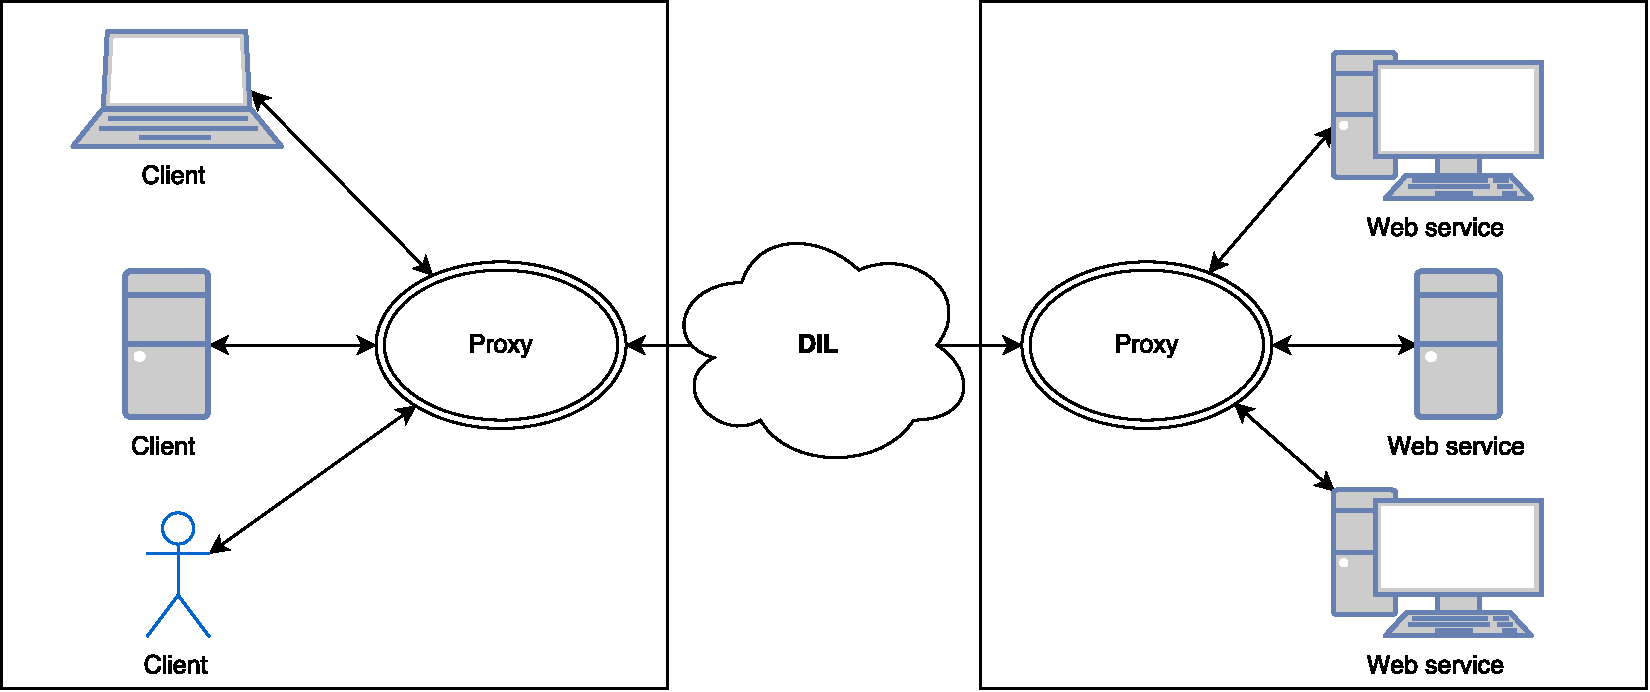
\includegraphics[scale=0.5]{images/proposed_solution.pdf}
\caption{Proposed proxy solution} \label{figure-proposed-proxy-solution}
\end{figure}

This approach is identified by IST-090 and is explored in this thesis. Based on
this recommendation we create a proxy with the aim of facilitating Web service
usage in DIL networks.


\section{Premises of the Thesis}

In this section we define the premises for the thesis and the proxy being
developed as a part of it. As we have previously discussed, W3C Web services are
in widespread use in NATO. Also the REST architectural style has been identified
as a technology of interest to NATO. As we discuss later in \cref{web-services},
\gls{http} is the by far most common transport protocol used by these types of
services. The first and second premise is therefore that the proxy must be able
to support both REST and W3C Web services deployed in a DIL network.

Next, in order to optimize Web services in DIL environments, the applications
themselves should not be required to be customized. All optimization should be
placed in proxies. This retains the interoperability with standards-based COTS
solutions. The fourth and final premise is that the proxy must work with standard
security mechanisms. In our case this means that any messages sent through the
proxies, must be exactly the same at the receiver as it would have been without
the proxies. This is due to both the header fields and the body of the message
can be part of security mechanisms, such as digital signatures and the presence
of authentication header fields.

To summarize, the premises of this thesis are that the proxy solution must:

\begin{enumerate}
    \item Support HTTP RESTful and W3C Web services.
    \item Work in DIL networks.
    \item Be interoperable with standards-based COTS solutions.
    \item Work with security mechanisms.
\end{enumerate}

\section{Scope and Limitations}

The goal of this thesis is to investigate optimization techniques for Web
services in \gls{dil} environments. We limit it to techniques that can be
applied at the application or the transport layer of the Internet protocol
suite (see \cref{figure-network-layers}). The reason for this is that NATO has
previously decided "everything over IP", a statement describing that all data
communication in NATO should occur with IP packets \cite{nnec-study}. We
therefore limit our optimization possibilities to the mentioned layers.

We mainly focus on the performance of Web services, yet security is of paramount
importance in military networks. Hence, any optimization techniques applied
should be possible to use together with common security mechanisms. Another
aspect is that applications that are to be used in military networks, need to be
approved by security authorities. If the application is too complex, e.g. it has
a very large code base or use a lot of external frameworks, the approval process
can be very lengthy. It is therefore an important consideration to make
the proxy as relatively simple as possible.


\section{Research Methodology}

Research is the systematic investigation of how to find answers to a specific
problem. It is broadly classified into \textit{Basic Research} and
\textit{Applied Research} \cite{rajasekar2006research}. Basic research, also
called fundamental or pure research, is research on basic principles and reasons
for occurrence of a particular event or process or phenomenon. It does not
necessarily have any practical use. Applied research, on the other hand, is
concerned about solving problems employing well known and accepted theories and
principles. In this thesis we set out to solve the actual real-world problem of
optimizing Web services, thus we perform applied science. To solve this problem
we need a systematic approach of how to perform the research. This is referred
to as \textit{research methodology} and says something about how the research is
to be carried out.

In this thesis we're performing research in the area of Computer Science, a
scientific discipline defined as \cite{denning}: \\

\textit{The systematic study of algorithmic processes that
describe and transform information: their theory, analysis, design, efficiency,
implementation, and application}.

\paragraph{}

 \citeauthor{denning} have identified three main processes for the computer science
 discipline, \textit{theory, abstraction} and \textit{design} \cite{denning}.
 \textit{Theory} derives from the mathematics discipline and applies to the areas of
 computer science that rely on underlying mathematics. Examples of this are
 the computer science areas of algorithms and data structures that involve
 complexity and graph theory. The next process, \textit{abstraction}, deals with
 modeling potential implementations. \textit{Design} is about the process of
 specifying a problem, transforming the problem statement into a design
 specification, and repeatedly inventing and investigating alternative solutions
 until a reliable, maintainable, documented, and tested design is achieved.

The research methodology used in this thesis is based on the design process. The
four steps and the efforts undertaken in them are summarized here:

\begin{description}

    \item[Specify the problem] The main focus of this thesis is how to improve
    the performance of Web services in DIL networks. We formulate a problem
    statement in \cref{section:problem-statement} and propose a possible
    solution in \cref{section:hypothesis}. Moreover, we present the technical
    background in \cref{chapter:background} and previous related work in
    \cref{chapter:related-work}.

    \item[Derive a design specification based on the requirements] Based on the
    premises, scope of the thesis, studies of the technological background and
    related work, we derive a set of requirements and specifications in
    \cref{chapter:requirements}.

    \item[Design and implement the system] When we identify the requirements for
    the optimization techniques, we design and implement them. This step is
    elaborated in \cref{chapter:design}.

    \item[Evaluate the system] Finally, the solution is evaluated through a
    series of tests. The purpose of this is to evaluate if we in fact were able
    to solve the problem we set out to solve. We cover the testing and
    evaluation in \cref{chapter:evaluation} and draw a conclusion in
    \cref{chapter:conclusion}.

\end{description}


\section{Contribution}

The outcome of this thesis is a recommendation regarding which optimizations
techniques can be used in DIL networks to increase the performance of Web
services. As a part of this work we implement a prototype DIL proxy.

\section{Outline}

The remainder of this thesis is organized as follows:

Chapter 2 presents the technical background for this thesis. We introduce
computer networks in general before we dive into different communication
paradigms and protocols. Then, in chapter 3, we discuss previous work done in
the area. In chapter 4 we derive a specification for the proxy, before we in
chapter 5 present the design and implementation details. Next, we present the
testing of the proxy and how the proxy fulfilled the premises and requirements
in chapter 6. Finally, in chapter 7, we summarize the discussion and provide
reflections on possible future work within this field.
